\chapter{EXPERIMENTS AND RESULTS}

\section{Introduction}
\hs This chapter presents the experimental results obtained from training and evaluating the crack segmentation models described in Chapter 3. The experiments were designed to address three primary research questions:
\begin{enumerate}
    \item How do different architectural paradigms (semantic segmentation, instance segmentation, and transformer-based models) compare in terms of crack detection accuracy and computational efficiency?
    \item Does the tile-based inference pipeline with blended overlap merging effectively preserve crack continuity when processing large-scale images?
    \item How well do models trained on public crack datasets generalize zero-shot to unseen, large-scale UAV imagery, and what does this imply for the deployment-time fine-tuning strategy?
\end{enumerate}

\hs The chapter begins by detailing the experimental environment and hardware specifications, followed by a summary of the dataset splits used for training, validation, and testing. Results are then presented for each model architecture, including performance metrics on public datasets, and inference pipeline evaluations.

\hs The evaluation is structured around two complementary settings. The first uses a held-out split of the aggregated public crack dataset described in Section~\ref{sec:data_acquisition}, which provides a controlled benchmark for comparing the three architectural paradigms under identical conditions. The second uses the CUBIT-InSeg UAV dataset as an external zero-shot test set, which introduces a deliberate domain shift and measures how well each model transfers to imagery that it has never seen during training. Reporting both settings allows the discussion in Chapter~\ref{chap:discussion} to separate gains attributable to architecture from gains attributable to data similarity.

\hs Three quantities are tracked throughout all experiments: segmentation accuracy, measured through IoU, precision, recall, and F1-score; inference latency, measured in milliseconds per image on a fixed consumer-grade GPU; and memory behaviour, including peak VRAM usage during tiled inference on large-scale images. Together, these three axes correspond directly to the deployment requirements established in Chapter~\ref{chap:introduction}: a model that is accurate but too slow to run on site, or fast but too imprecise to trust, is of limited practical value for infrastructure inspection.

\newpage

\section{Experimental Environment and Hardware Specifications}
\label{sec:experimental_environment_and_hardware_specifications}

\hs All experiments used a consistent hardware and software environment. The training environment was a Google Colab instance with a Tesla T4 GPU, while the evaluation environment was a local machine. Specifications are summarized in Table \ref{tab:hardware_specs}.

\begin{table}[htbp]
    \centering
    \caption{\textit{Experimental hardware and software specifications}}
    \label{tab:hardware_specs}
    \begin{tabular}{l p{0.75\textwidth}}
        \toprule
        \textbf{Component}       & \textbf{Specification}                   \\
        \midrule
        \multicolumn{2}{l}{\textit{Training Environment (Google Colab)}}    \\
        \midrule
        RAM                      & 12 GB                                    \\
        GPU                      & NVIDIA Tesla T4 (16 GB)                  \\
        CUDA Cores               & 2560                                     \\
        \multicolumn{2}{l}{\textit{Evaluation Environment (Local Machine)}} \\
        \midrule
        CPU                      & 11th Gen Intel Core i7-11800H @ 2.30 GHz \\
        RAM                      & 16 GB                                    \\
        GPU                      & NVIDIA GeForce GTX 1650 (4 GB)           \\
        \multicolumn{2}{l}{\textit{Software Stack}}                         \\
        \midrule
        Operating System         & 64-bit operating system                  \\
        Python Version           & 3.11.15                                  \\
        PyTorch Version          & 1.10.0                                   \\
        CUDA Version             & 11.8                                     \\
        cuDNN Version            & 8.2.1                                    \\
        \bottomrule
    \end{tabular}
\end{table}

\hs The Tesla T4 GPU (16 GB VRAM) provided sufficient resources for training with reasonable batch sizes. Inference on large-scale images, however, was performed on a local NVIDIA GeForce GTX 1650 (4 GB VRAM), which imposed significant limitations: batch sizes were restricted to 2--4 samples, and high-resolution processing required the tile-based pipeline described in Section \ref{sec:evaluation_framework}. These constraints are representative of edge-deployment scenarios.

\hs All three models were trained using mixed-precision (AMP), as configured in Table \ref{tab:training-hyperparameters}. For U-Net and SegFormer, the best-performing checkpoint was selected based on validation IoU. For YOLO26s-seg, the best checkpoint was selected based on validation mAP50-95, with early stopping triggered at epoch 92.

\hs The software stack was selected for compatibility with the segmentation frameworks used in this study. PyTorch 1.10.0 provided the foundation for the Segmentation Models PyTorch (SMP) framework, which supplied the U-Net and SegFormer implementations. YOLO26s-seg was trained using the Ultralytics framework. All models were exported to ONNX format at opset 18 for deployment, as described in Section \ref{subsec:model_export}. Inference on the local GTX 1650 was performed exclusively through the ONNX models.

\newpage

\hs Figure \ref{fig:training_validation_loss} shows the training and validation loss curves for all three models. U-Net and SegFormer both converged smoothly, reaching their best validation IoU at epochs 45 and 47 respectively. YOLO26s-seg reached its best validation mAP50-95 at epoch 62 and triggered early stopping at epoch 92. In all three cases, the curves track closely, indicating no significant overfitting.

\begin{figure}[H]
    \centering
    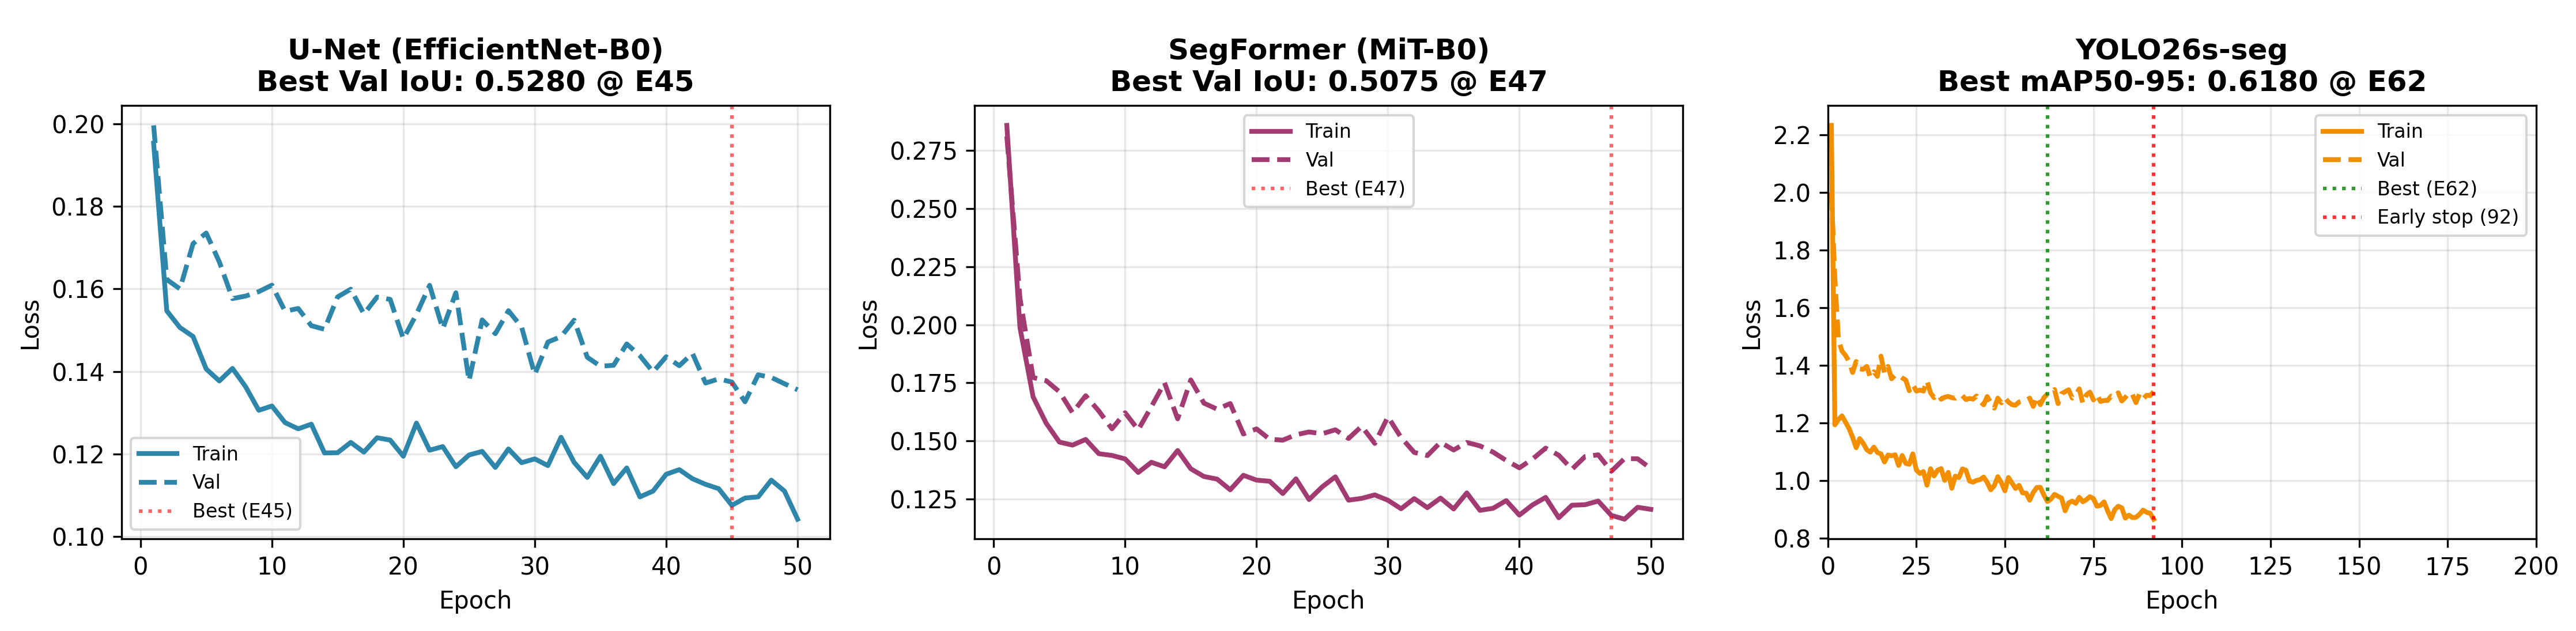
\includegraphics[width=\textwidth]{figures/plots/training_validation_loss.png}
    \caption{Training and validation loss curves for U-Net (left), SegFormer (middle), and YOLO26s-seg (right). Dashed vertical lines mark the best epoch and early stop point for each model.}
    \label{fig:training_validation_loss}
\end{figure}

\section{Results from Baseline Architectures}
\label{sec:results_from_baseline_archtectures}

\subsection{Performance on Public Datasets}
\label{subsec:performance_on_public_datasets}

\hs Each model was trained using the protocol described in Section \ref{sec:model_development_and_selection} and evaluated on the held-out test split (882 images). Performance metrics are reported at the optimal threshold determined via validation set analysis.

\begin{figure}[htbp]
    \centering
    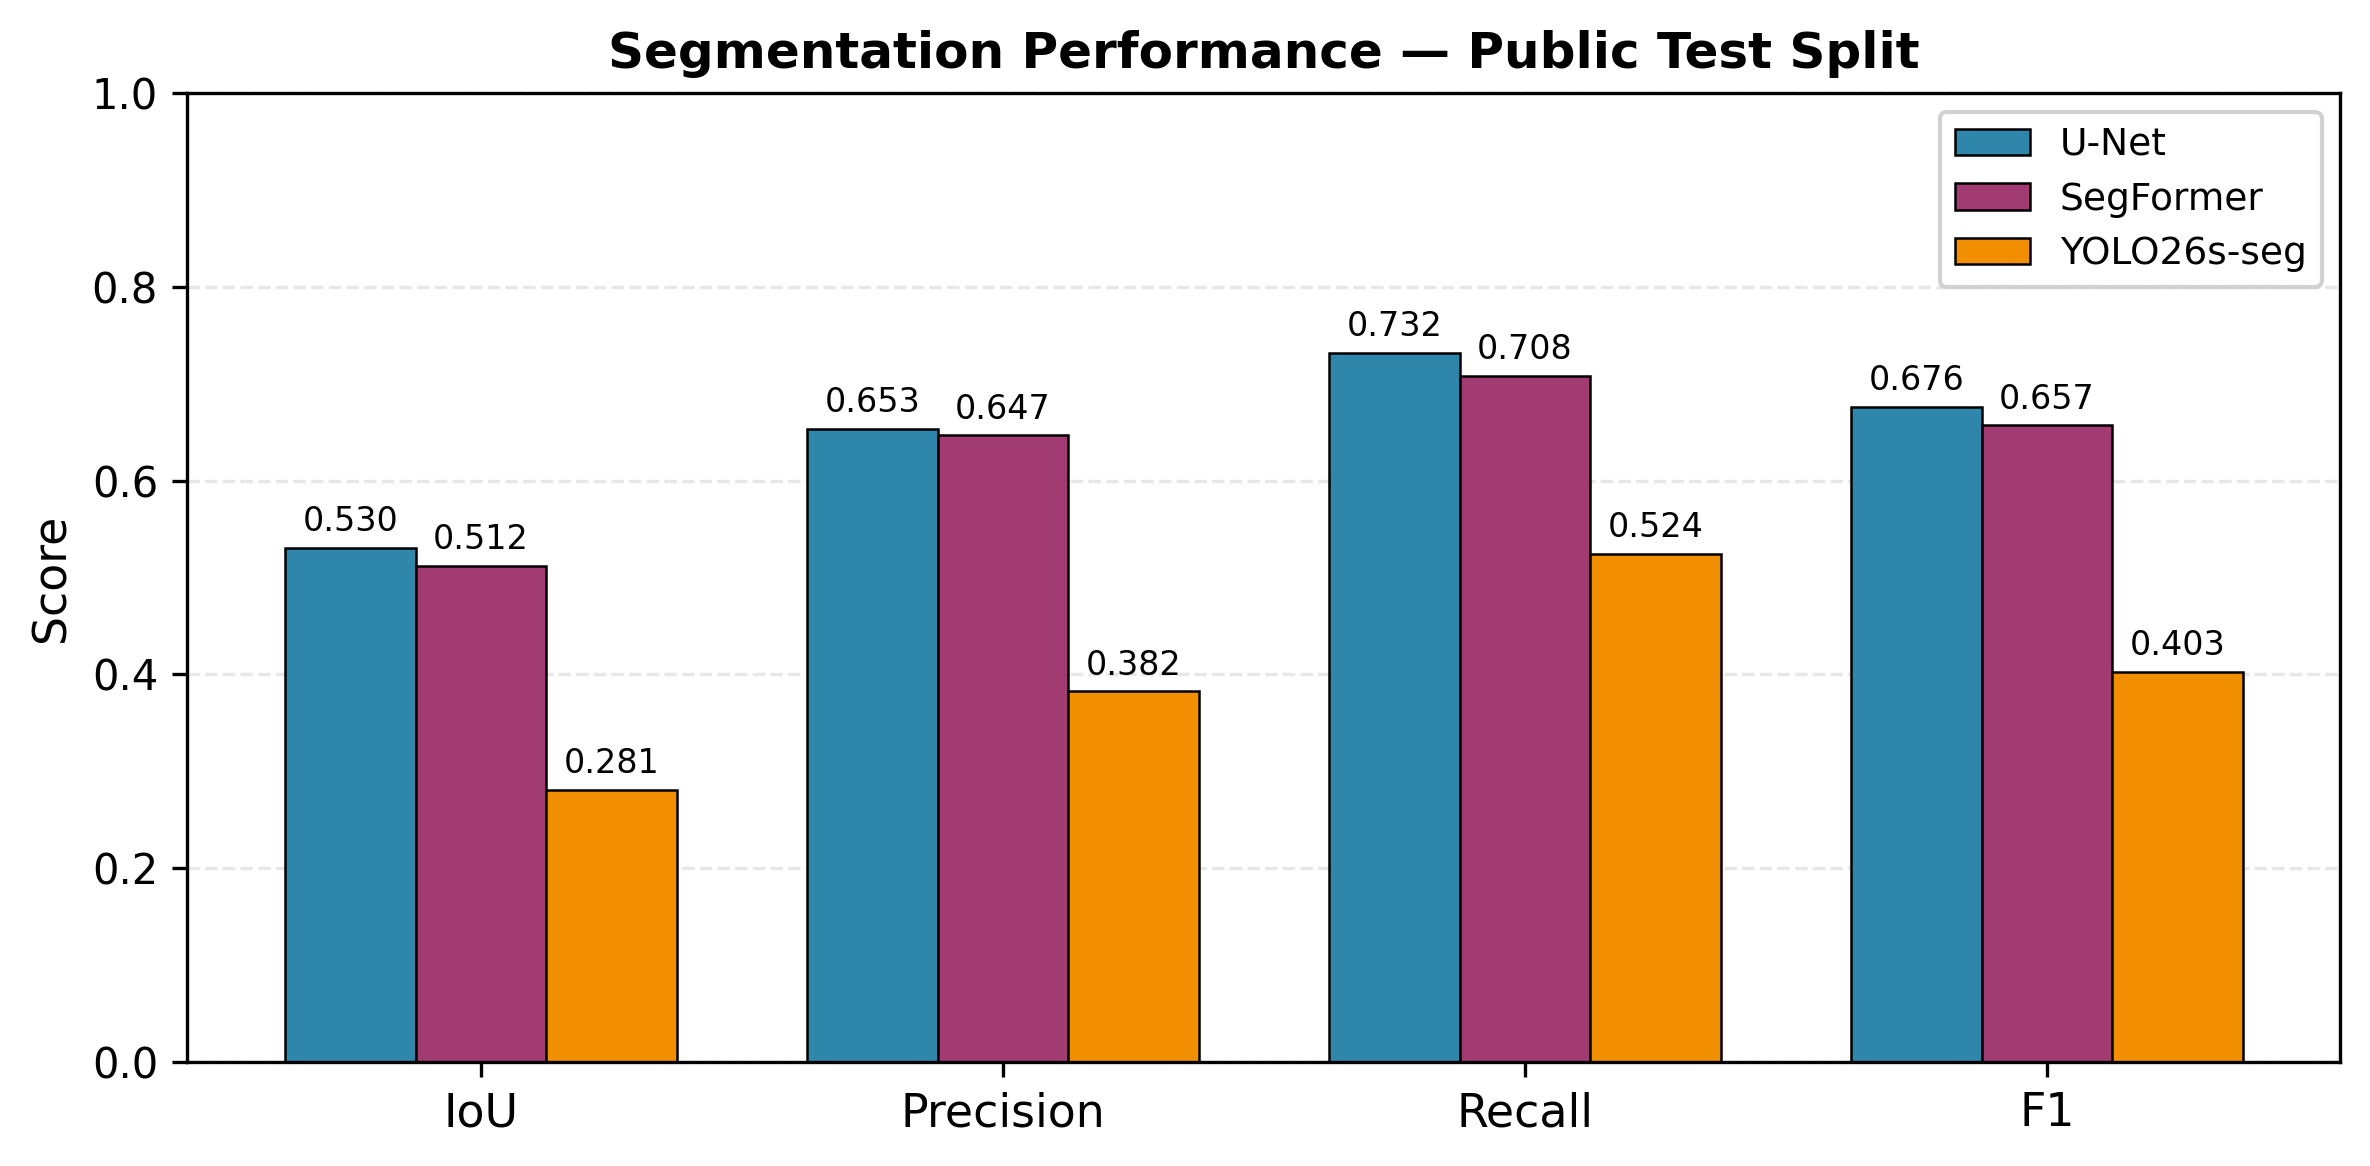
\includegraphics[width=\textwidth]{figures/plots/metrics_on_public_test.png}
    \caption{\textit{Segmentation performance on the public test split (882 images).}}
    \label{fig:metrics_on_public_test}
\end{figure}

\hs Figure \ref{fig:metrics_on_public_test} visualizes these results across the four primary metrics, confirming that U-Net leads in IoU, precision, and F1-score, with SegFormer
closely matching its performance. At first glance, YOLO26s-seg trails substantially in every accuracy metric despite being approximately 4.7× faster at inference.

\begin{table}[htbp]
    \centering
    \caption{\textit{Segmentation performance on test split}}
    \label{tab:segmentation_performance}
    \begin{tabular}{lccccc}
        \toprule
        \textbf{Model} & \textbf{IoU}    & \textbf{P}      & \textbf{R}      & \textbf{F1}     & \textbf{Time (ms)} \\
        \midrule
        U-Net          & \textbf{0.5304} & \textbf{0.6532} & \textbf{0.7316} & \textbf{0.6759} & 84.45              \\
        SegFormer      & 0.5121          & 0.6467          & 0.7084          & 0.6570          & 75.96              \\
        YOLO26s-seg    & 0.2810          & 0.3823          & 0.5243          & 0.4026          & \textbf{18.07}     \\
        \bottomrule
    \end{tabular}
\end{table}

\hs Table \ref{tab:segmentation_performance} compares the performance of U-Net, SegFormer, and YOLO26s-seg for crack segmentation. U-Net achieved the highest overall segmentation performance, with an IoU of 53.04\%, precision of 65.32\%, recall of 73.16\%, and F1-score of 67.59\%. This indicates that U-Net was the most effective at capturing crack regions and producing accurate segmentation masks.

\hs SegFormer produced comparable results, achieving an IoU of 51.21\% and an F1-score of 65.70\%, while being slightly faster than U-Net (75.96 ms versus 84.45 ms). Thus, SegFormer provides a good balance between segmentation accuracy and inference speed.

\hs YOLO26s-seg was considerably faster, with an inference time of 18.07 ms, but its segmentation performance was substantially lower, with an IoU of 28.10\% and an F1-score of 40.26\%. This demonstrates a clear trade-off between speed and segmentation accuracy.

\hs Overall, for this dataset, U-Net was the best-performing model for crack segmentation, while SegFormer offered a competitive balance between accuracy and speed. YOLO26s-seg was the fastest model but produced less accurate segmentation results.

\section{Results and Analysis on Large Scale Images}
\label{sec:results_and_analysis_on_large_scale_images}

\subsection{Model Adaptation and Performance}
\label{subsec:model_adaptation_and_performance}

\hs All models were evaluated on CUBIT-InSeg in a zero-shot setting: they were trained only on the public datasets described in Section \ref{subsec:public-datasets} and were not fine-tuned on CUBIT-InSeg. This setting was chosen deliberately, as it mirrors the first deployment of the model to a new aenvironment, where no site-specific training data is yet available (see Section \ref{sebsec:cubit-for-zero-shot}).

\begin{figure}[htbp]
    \centering
    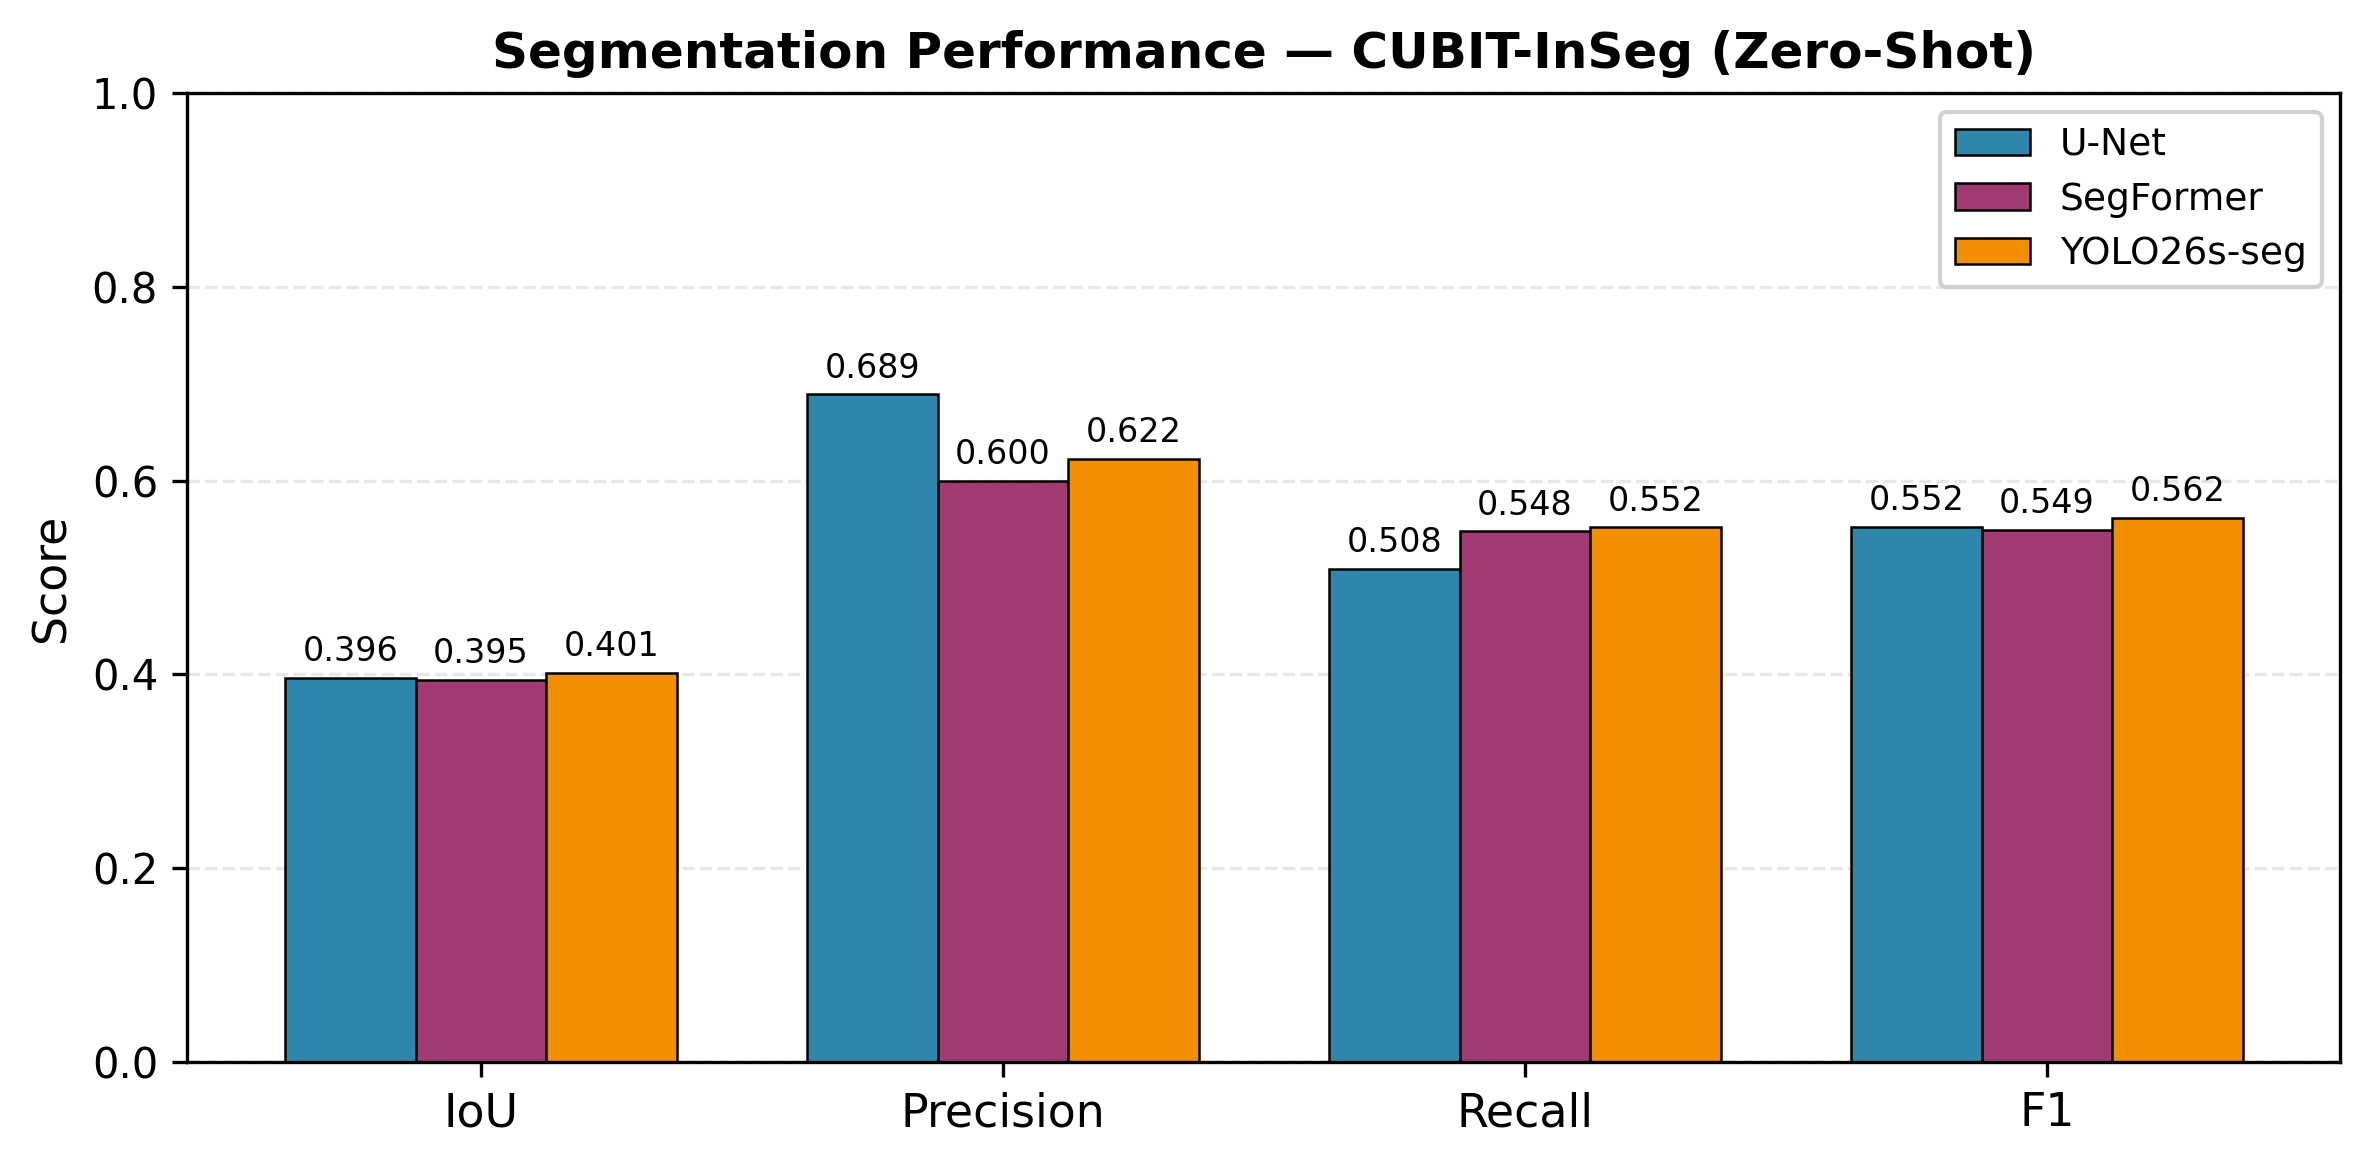
\includegraphics[width=\textwidth]{figures/plots/metrics_on_cubit.png}
    \caption{\textit{Zero-shot segmentation performance on CUBIT-InSeg.}}
    \label{fig:metrics_on_cubit_inseg}
\end{figure}

\newpage

\hs Figure \ref{fig:metrics_on_cubit_inseg} visualizes zero-shot results, highlighting how the performance gap between models narrows substantially on CUBIT-InSeg compared to the public split. All three architectures converge to comparable IoU and F1-score values under domain shift, with YOLO26s-seg marginally leading.

\begin{table}[htbp]
    \centering
    \caption{\textit{Segmentation performance on CUBIT-InSeg test dataset}}
    \label{tab:cubit_inseg_performance}
    \begin{tabular}{lccccc}
        \toprule
        \textbf{Model} & \textbf{IoU}    & \textbf{Precision} & \textbf{Recall} & \textbf{F1}     & \textbf{Time (ms)} \\
        \midrule
        U-Net          & 0.3962          & \textbf{0.6890}    & 0.5085          & 0.5521          & 4903.53            \\
        SegFormer      & 0.3946          & 0.5995             & 0.5476          & 0.5488          & 5188.30            \\
        YOLO26s-seg    & \textbf{0.4012} & 0.6222             & \textbf{0.5518} & \textbf{0.5616} & \textbf{3940.39}   \\
        \bottomrule
    \end{tabular}
\end{table}

\hs Table \ref{tab:cubit_inseg_performance} summarizes results on CUBIT-InSeg, a large-scale dataset with higher-resolution images and cracks traversing tile boundaries, providing a stress test for both segmentation accuracy and the tile-based pipeline. Although IoU values dropped compared to the public test split (Table \ref{tab:segmentation_performance}), this is expected given the increased resolution, crack variation, and complex backgrounds. Among the three models, YOLO26s-seg achieved the highest IoU (40.12\%) and F1-score (56.16\%), closely followed by U-Net (IoU 39.62\%, F1 55.21\%) and SegFormer (IoU 39.46\%, F1 54.88\%).

\hs In precision and recall, U-Net led at 68.90\% precision (fewest false positives), while SegFormer achieved the acceptable recall (54.76\%) at the cost of lower precision (59.95\%). YOLO26s-seg sat in the middle (precision 62.22\%, recall 55.18\%), yielding the most balanced F1-score.

\newpage

\hs Inference times on CUBIT-InSeg ranged from 3,940.39 ms (YOLO26s-seg) to 5,188.30 ms (SegFormer), a substantial increase over the public split due to tile-wise processing. Notably, U-Net (4,903.53 ms) became faster than SegFormer, and YOLO26s-seg retained its speed advantage, though it no longer translates into meaningful segmentation improvement.

\hs The zero-shot results on CUBIT-InSeg should be interpreted as a lower bound on the model's expected performance in deployment. In the intended workflow, a small number of images collected from the customer's site would be used to fine-tune the model before full-scale inference, which is expected to close part of the domain gap observed here. Quantifying the gains from such deployment-time fine-tuning is left as future work (Section \ref{sec:future_work}).

\subsection{Generalization to Unseen Large-Scale Data}
\label{subsec:generalization_to_unseen_large_scale_data}

\hs Figure \ref{fig:cubit_inseg_comparison} presents a qualitative comparison of the three models on the CUBIT-InSeg dataset. The results demonstrate that while all models face challenges with crack continuity across tile boundaries, U-Net produces the most coherent segmentation masks, particularly in regions with fine crack structures are blended with the surrounding background. Also, SegFomer shows a balanced performance, as it does not lose the crack topology and continuity as much as YOLO26s-seg. YOLO26s-seg, while faster, exhibits more discontinuities in regions with varying crack intensity, leading to fragmented segmentation outputs.

\begin{figure}[htbp]
    \centering
    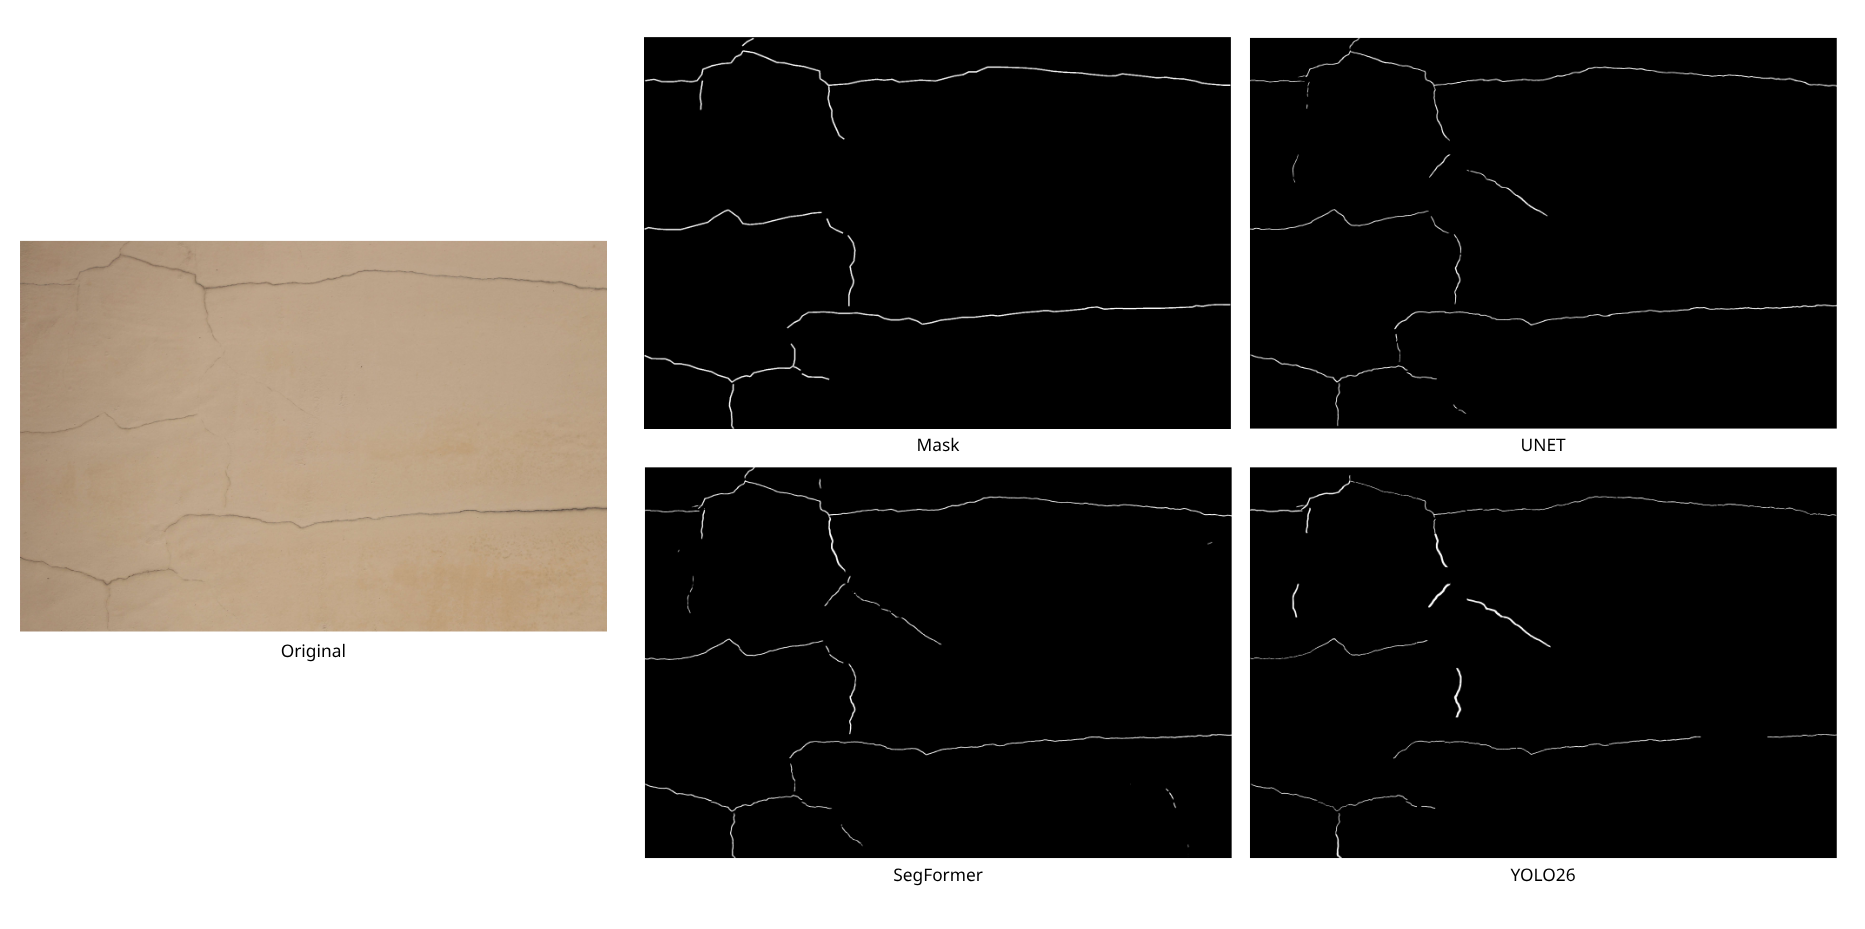
\includegraphics[width=\textwidth]{figures/cracks/CUBIT-InSeg Model Comparison.png}
    \caption{\textit{Qualitative comparison on the CUBIT-InSeg dataset.}}
    \label{fig:cubit_inseg_comparison}
\end{figure}

\hs The tile-based inference pipeline with blended overlap merging effectively preserves crack continuity across tile boundaries, as evidenced by the smooth transitions in the merged outputs. However, some discontinuities remain visible in regions where crack intensity varies significantly across tiles, particularly for YOLO26s-seg. Additionally, for SegFormer, the model occasionally misclassifies background textures as cracks, leading to false positives in the segmentation masks. However, the model demnonstrated a balance performance as it does not lose the crack topology and continuity as much as YOLO26s-seg.

\hs Overall, U-Net remains the more reliable model for crack segmentation in large-scale images, while YOLO26s-seg offers faster inference at the cost of reduced accuracy

\section{Summary}
\label{sec:summary}

\hs This chapter presented the experimental results of training and evaluating three crack segmentation architectures, U-Net (EfficientNet-B0), SegFormer (MiT-B0), and YOLO26s-seg, under a unified protocol. The key findings are summarized as follows:

\textbf{Performance on Public Datasets (Table \ref{tab:segmentation_performance}):} U-Net achieved the highest segmentation accuracy with an IoU of 53.04\% and F1-score of 67.59\%, followed closely by SegFormer (IoU 51.21\%, F1 65.70\%). YOLO26s-seg was the fastest model (18.07 ms) but produced substantially lower segmentation quality (IoU 28.10\%, F1 40.26\%). This confirms a clear trade-off between inference speed and segmentation accuracy for crack detection.

\textbf{Zero-Shot Generalization to Large-Scale UAV Imagery (Table \ref{tab:cubit_inseg_performance}):} On the unseen CUBIT-InSeg dataset, all models experienced a performance drop, as expected given the domain shift and increased image resolution. YOLO26s-seg achieved the highest IoU (40.12\%) and F1-score (56.16\%), narrowly outperforming U-Net (IoU 39.62\%, F1 55.21\%) and SegFormer (IoU 39.46\%, F1 54.88\%). U-Net maintained the highest precision (68.90\%), indicating fewer false positives, while SegFormer showed balanced recall. Inference times increased substantially due to tile-wise processing, ranging from 3,940 ms (YOLO26s-seg) to 5,188 ms (SegFormer).

\textbf{Tile-Based Inference Pipeline:} The sliding window approach with 25\% overlap and blended merging effectively preserved crack continuity across tile boundaries, as demonstrated by the qualitative results in Figure \ref{fig:cubit_inseg_comparison}. U-Net produced the most coherent segmentation masks, while YOLO26s-seg showed some discontinuities in regions with varying crack intensity. SegFormer occasionally misclassistatisticsfied background textures as cracks, leading to false positives.